\documentclass{article}

\usepackage[spanish]{babel}
\usepackage{amsmath}
\usepackage{txfonts}
\usepackage[boxed]{algorithm2e}
\usepackage{amssymb}
\usepackage[pdftex]{graphicx}
\usepackage[utf8x]{inputenc}
\usepackage{enumerate}
\usepackage{url}
\DeclareGraphicsExtensions{.jpg, .png, .mps, .bmp, .pdf}
\usepackage{epsfig}
\usepackage{subfigure}
\newtheorem{Definition}{Definition} 
\newtheorem{Example}{Example} 
\newtheorem{Theorem}{Theorem} 
\newtheorem{Proof}{Proof} 
\newcommand{\denselist}{\topsep 0pt \itemsep -4pt}
\newcommand{\tup}[1]{\langle #1 \rangle}
\newcommand{\vvec}[1]{\mathbf{#1}}
\newcommand{\join}{\bowtie}
\newcommand{\R}{\mathcal{R}}
\newcommand{\Q}{\mathcal{Q}}
\newcommand{\body}{{body}}
\newcommand{\head}{{head}}
\newcommand{\qrule}{:\!\!-}
\newcommand{\arc}{\text{arc}}
\newcommand{\Theory}[1]{T(#1)}
\newcommand{\Omit}[1]{}
\newcommand{\citeX}[1]{\citeauthor{#1}~\citeyear{#1}}

\newcommand{\minicon}{{MiniCon}}
\newcommand{\mcdsat}{\textsc{McdSat}}

\begin{document}

\begin{titlepage}

\begin{flushleft}
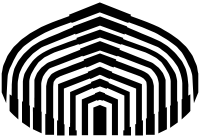
\includegraphics[scale=0.3]{graphics/logo_usb.png} \\
Universidad Simón Bolívar \\
Coordinación de Ciencias de la Computación \\
Maestría en Ciencias de la Computación \\
\end{flushleft}

\vspace{0.8cm}

\begin{center}
{\large \bf \textsf{Instanciación Óptima de Flujos de Trabajo Abstractos Usando Lógica y Circuitos}}
\end{center}

\vspace{0.2cm}

\begin{abstract}
Una arquitectura orientada a servicios típica se separa en dos capas --grupos de
componentes-- principales.
La capa concreta con servicios concretos cuyas funcionalidades son descritas en
términos de pre- y post-condiciones y propiedades no funcionales en términos de
parámetros de calidad de servicio (Quality Of Service, QoS), y la capa abstracta
con aplicaciones de software cuyas funcionalidades son descritas en términos de
flujos de trabajo abstractos y propiedades no funcionales en términos de
restricciones sobre QoS. Durante la ejecución de un flujo de trabajo o \emph{workflow}, los
servicios abstractos son instanciados en servicios concretos que cumplen con los
requerimientos funcionales y no funcionales. Esta instanciación, que debe ser
hecha en el momento, consiste de una búsqueda en un espacio de posibilidades
combinatorio. En este trabajo se propone una infraestructura para resolver
eficientemente el problema de instanciación que está basada en
la lógica proposicional. La infraestructura adopta el enfoque de definición denominado Local-As-View en la cual la
funcionalidad de servicios concretos se describe usando vistas de servicios
abstractos, la calidad de una instanciación como una función de utilidad global
que combina los diferentes parámetros QoS, y los flujos de trabajo abstractos
como consultas conjuntivas sobre servicios abstractos. Usando esta
representación, el problema de instanciación de flujos de trabajo se convierte
en un problema de reescritura de consultas, del área de sistemas de integración.
Entonces, en base a enfoques reportados en la literatura, se propone una codificación del
problema de instanciación de flujos de trabajo como una teoría lógica cuyos
modelos están en correspondencia con las instanciaciones del flujo de trabajo, y
los modelos mejor calificados en correspondencia con instanciaciones óptimas del
flujo de trabajo. Así, explotando propiedades conocidas de teorías lógicas en
formato d-DNNF, se provee una solución eficiente y escalable al problema de
instanciación de flujos de trabajo. Esta solución no sólo escala a
instancias grandes como muestran resultados experimentales ya realizados, sino
que también podemos verificar que es correcta y completa dado que, estando basada en la lógica, es
fácilmente sujeta al análisis formal.
\end{abstract}

\vspace{\fill}

\begin{minipage}{0.3\textwidth}
\begin{flushleft}
\emph{Estudiante:} \\
Daniel \textsc{Izquierdo} \\
Carnet 08-86809 \\
\end{flushleft}
\end{minipage}
\begin{minipage}{0.3\textwidth}
\begin{center}
Fecha estimada de culminación: \\
Marzo de 2010
\end{center}
\end{minipage}
\begin{minipage}{0.3\textwidth}
\begin{flushright}
\emph{Asesores:} \\
Prof. Blai \textsc{Bonet} \\
Prof. María Esther \textsc{Vidal} \\
\end{flushright}
\end{minipage}

\end{titlepage}


\tableofcontents
\newpage

\section{Planteamiento del Problema}

En el contexto de la Web Semántica, y con el soporte de las Arquitecturas Orientadas a
Servicios (SOA), el número de fuentes de datos y servicios Web ha explotado en
los últimos años. Por ejemplo, la colección de bases de datos de biología
molecular actualmente contiene 1.170 bases de datos~\cite{Galperin09}, un número
que es
mayor que el del último año por 95~\cite{Galperin2008}, y que el de hace dos
años por 110~\cite{Galperin2007};
las herramientas y servicios, así como el número de instancias
publicados por estos recursos, siguen una progresión similar~\cite{Benson07}.
Gracias a
esta variedad de datos, la tendencia de los usuarios es hacia depender cada vez
más de métodos automáticos para manejarlos tales como recuperación de datos de
fuentes públicas y análisis utilizando herramientas o servicios Web compuestos
en flujos de trabajo complejos.

La SOA típica consiste de dos capas. La capa concreta que está hecha de
servicios concretos cuyas funcionalidades son descritas en términos de pre- y
post-condiciones y propiedades no funcionales en conjuntos de parámetros de
calidad de servicio (QoS), y
la capa abstracta compuesta de aplicaciones de software cuyas funcionalidades
son descritas en términos de flujos de trabajo abstractos y propiedades no
funcionales en términos de restricciones de QoS. La ejecución de un flujo de
trabajo abstracto involucra la instanciación de los servicios abstractos en
servicios concretos que cumplan con los requerimientos funcionales y no
funcionales. Este proceso de instanciación puede ser visto como una búsqueda de
una instanciación objetivo en el espacio combinatorio de todas las
instanciaciones válidas. Entonces se está interesado en técnicas eficientes para
realizar esta búsqueda que sean capaces de escalar a medida que el número de
servicios concretos o la complejidad (número
de objetivos, tamaño) de la estructura del flujo de trabajo  aumenta. Se llama al
problema de instanciar un flujo de trabajo dado con servicios concretos de un
conjunto de servicios concretos dado, de manera que ciertas restricciones sobre QoS sean
cumplidas, el Problema de Instanciación de Flujos de Trabajo (WIP).

En este trabajo se considera una versión restringida de WIP que adopta el
enfoque Local-As-View (LAV) \cite{levy:bucket}. En LAV, todos los elementos de un
problema son especificados con un lenguaje común basado en servicios abstractos
tal que los servicios concretos se describen como vistas de servicios
abstractos, la calidad de una instanciación como una función de utilidad global
que combina los diferentes parámetros QoS, y el flujo de trabajo abstracto como
una consulta conjuntiva sobre los servicios abstractos; esta representación es
similar a la que es generada de manera semiautomática para el sistema DEIMOS
\cite{AmbiteISWC09}. En esta versión de WIP, las reglas que definen flujos de trabajo
(consultas conjuntivas) y servicios concretos (vistas) son creados de manera que
todas las restricciones funcionales sobre pre- y post-condiciones de los
servicios y sus combinaciones sean satisfechas, y las medidas de QoS son
representadas anotando cada descripción de servicio concreto con un número real
que representa la utilidad QoS global del servicio.

Bajo estas suposiciones, WIP puede ser convertido en el bien conocido Problema
de Reescritura de Consultas (QRP) para LAV que es central a los sistemas de
integración \cite{halevy:survey}. QRP consiste de una consulta conjuntiva que debe ser
respondida en términos de vistas donde la consulta y las vistas son descritas
usando LAV con relaciones abstractas. Este problema es importante en el contexto
de integración de datos \cite{Chen05,JaudoinPRST05}, y optimización de consultas y mantenimiento
de datos \cite{AfratiLU07,levy:bucket}, y varias soluciones que escalan a un número grande de
vistas han sido definidas \cite{arvelo:aaai06,pods:DuschkaG97,sac:DuschkaG97,levy:bucket,pottinger:minicon}.

La solución propuesta por Arvelo et al. \cite{arvelo:aaai06} está basada en la enumeración
eficiente de modelos de una teoría lógica proposicional. Dada una consulta conjuntiva
y un conjunto de fuentes definidas como vistas, se construye una teoría
lógica de manera que cada modelo de la teoría codifica una
reescritura válida, y así todas las reescrituras son obtenidas enumerando los
modelos de la teoría. Esta enumeración puede ser realizada eficientemente si la
teoría lógica está en cierta forma normal llamada la forma normal de negación
determinística y descomponible (d-DNNF) \cite{darwiche:d-dnnfs}. Así,
la solución consiste en transformar (llamado compilar en el campo de
compilación del conocimiento) la teoría lógica en el formato d-DNNF para
enumerar sus modelos eficientemente.

Pero las teorías d-DNNF no sólo soportan la enumeración eficiente de sus
modelos, sino también otras operaciones. Entre ellas se encuentra la enumeración
de los modelos con mejor calidad. Dada una función de calidad de literales
$r(\ell)$ que asigne calidades a cada literal $\ell$, se define la calidad
$r(\omega)$ de un modelo $\omega$ como la suma de las calidades de los literales
activados por $\omega$ (es decir,
$r(\omega)\doteq\sum_{\omega\vDash\ell}r(\ell)$), y se dice que $\omega$ es un modelo
de mejor calidad si no hay modelo $\omega'$ tal que $r(\omega')<r(\omega)$.

Dada una teoría en d-DNNF, se computa la calidad de los mejores modelos, y
los mejores modelos, en tiempo lineal en el tamaño del d-DNNF. Este cómputo
transforma el GAD del d-DNNF en un circuito aritmético reemplazando los nodos
AND con `+' y los nodos OR con `min'. La función de calidad de literales
asigna valores a las hojas del circuito aritmético (grafo acíclico dirigido usado
para calcular polinomios) que son propagados a la raíz en tiempo
lineal. El valor de la raíz es la calidad del mejor modelo \cite{darwiche:weighted}.

En este trabajo se propone explotar las propiedades de los d-DNNF construyendo una
teoría lógica cuyos modelos codifican las instanciaciones del flujo de trabajo
y cuyos mejores modelos codifican las instanciaciones óptimas (mejores). Así, la
búsqueda combinatoria se reduce a la computación de un mejor modelo de una
teoría lógica que puede ser realizada eficientemente una vez que la teoría es
transformada al formato d-DNNF.

\subsection{Ejemplo Motivante}

% flights
\newcommand{\vuelo}{\text{\it vuelo}}
\newcommand{\ciudadVE}{\text{\it ciudadVE}}
\newcommand{\nacional}{\text{\it nacional}}
\newcommand{\ida}{\text{\it ida}}
\newcommand{\unaescala}{\text{\it una-escala}}
\newcommand{\vueloCCS}{\text{\it vuelo-hacia-ccs}}
\newcommand{\unaparadaCCS}{\text{\it unaescala-hacia-ccs}}
\newcommand{\desdeVAL}{\text{\it desde-val}}
\newcommand{\PA}{\text{CCS}}
\newcommand{\NY}{\text{VAL}}
\newcommand{\AL}{\text{AL}}
% end flights

Considere un sistema simple de información de vuelos que contiene información
sobre vuelos entre ciudades e información sobre qué ciudades están en los
Estados Unidos. Un sistema así puede ser descrito usando LAV con los dos servicios
abstractos $\vuelo(x,y)$ y $\ciudadVE(x)$. El primero relaciona dos ciudades $x$ e $y$ si
hay un vuelo directo entre ellas, y el segundo dice si $x$ es una ciudad de
Venezuela  o no. Para los servicios concretos, supongamos que las fuentes de
datos disponibles en Internet contienen la siguiente información:

\begin{enumerate}[--]
\item $\nacional(x,y)$ relaciona dos ciudades de Venezuela conectadas por un vuelo directo,
\item $\ida(x,y)$ relaciona dos ciudades conectadas por un vuelo de ida,
\item $\unaescala(x,y)$ relaciona dos ciudades conectadas por un vuelo con una escala,
\item $\vueloCCS(x)$ dice si hay un vuelo directo desde $x$ a Caracas,
\item $\unaparadaCCS(x,y)$ relaciona $x$ y $y$ si hay un vuelo desde $x$ a Caracas con una escala en $y$, y
\item $\desdeVAL(x)$ dice si hay un vuelo de Valencia a $x$.
\end{enumerate}

Adicionalmente, los servicios concretos se describen con los siguientes
servicios abstractos:

\begin{alignat*}{1}
\nacional(x,y)\   &\qrule\ \vuelo(x,y),\,\ciudadVE(x),\,\ciudadVE(y)\,. \\
\ida(x,y)\     &\qrule\ \vuelo(x,y)\,. \\
\unaescala(x,z)\    &\qrule\ \vuelo(x,y),\,\vuelo(y,z)\,. \\
\vueloCCS(x)\     &\qrule\ \vuelo(x,\PA)\,. \\
\unaparadaCCS(x,y)\  &\qrule\ \vuelo(x,y),\,\vuelo(y,\PA)\,. \\
\desdeVAL(x)\       &\qrule\ \vuelo(\NY,x)\,.
\end{alignat*}

Ahora supongamos que un usuario está interesado en construir una aplicación
capaz de recuperar los vuelos ida y vuelta con una parada hacia cualquier ciudad
en el mundo, tales que los vuelos puedan detenerse en cualquier ciudad.

\[ W(x,w,y,z) \qrule \ciudadVE(x),\,\vuelo(x,w),\,\vuelo(w,y),\,\vuelo(y,z),\,\vuelo(z,x)\,. \]

La siguiente consulta conjuntiva representa el flujo de trabajo que define esta
solicitud en términos de servicios abstractos. El flujo de trabajo es definido
de manera que todo lo relacionado sobre el ligamiento de parámetros de
entrada/salida es resuelto. Así, cualquier instanciación de los servicios
abstractos en términos de los servicios concretos es una implementación válida
del flujo de trabajo. Las implementaciones corresponden a composiciones de
servicios concretos en las cuales un servicio concreto puede implementar uno o
más servicios abstractos del flujo, pero cada servicio abstracto puede ser
implementado por exactamente un servicio concreto. Por ejemplo, la siguiente
composición corresponde a una de estas implementaciones.

\[ I(x,w,y,z)\ \qrule\ \nacional(x,w),\,\vueloCCS(w),\,\ida(\PA,z),\,\nacional(z,x)\,. \]

Sin embargo, las siguientes dos composiciones no son válidas.

\begin{alignat*}{1}
I'(x,w,y,z)\  \qrule\ &\nacional(x,y),\,\vueloCCS(y),\,\desdeVAL(z),\,\nacional(z,x)\,. \\
I''(x,w,y,z)\ \qrule\ &\unaescala(x,y),\,\ida(y,z),\,\nacional(z,x)\,.
\end{alignat*}

La primera composición no es válida porque asocia la variable del flujo $y$ a
las constantes \PA\ y \NY\ que denotan ciudades diferentes. En la otra mano, $I''$
no lo implementa porque el servicio concreto $\unaescala(x,y)$ no recibe como entrada
o produce como salida la ciudad intermedia donde el vuelo se detiene y entonces
no es posible asegurarse de que esa ciudad esté asociada a la ciudad $w$ que es
retornada por el flujo de trabajo.

Estos ejemplos muestran que las instanciaciones correctas de un flujo deben
manejar constantes de manera que dos constantes distintas no sean asociadas
entre sí de manera directa o indirectamente vía transitividad, y que todos los
atributos que aparezcan en un \emph{join} o en la salida sean producidos por los
servicios concretos seleccionados.

Los parámetros QoS son modelados anotando los servicios concretos con utilidades
que caracterizan su comportamiento y que luego son agregados durante la
instanciación. Así, como se mencionó previamente, la mejor instanciación es la
que minimiza (o maximiza) la agregación de utilidades.

\section{Justificación e importancia}

\subsection{Ejemplo motivante}

% flights
\newcommand{\flight}{\text{\it flight}}
\newcommand{\UScity}{\text{\it uscity}}
\newcommand{\national}{\text{\it national}}
\newcommand{\oneway}{\text{\it one-way}}
\newcommand{\onestop}{\text{\it one-stop}}
\newcommand{\flightPA}{\text{\it flight-to-pa}}
\newcommand{\onestopPA}{\text{\it onestop-to-pa}}
\newcommand{\fromNY}{\text{\it from-ny}}
\newcommand{\PA}{\text{PA}}
\newcommand{\NY}{\text{NY}}
\newcommand{\AL}{\text{AL}}
% end flights

Considere un sistema simple de información de vuelos que contiene información
sobre vuelos entre ciudades e información sobre qué ciudades están en los
Estados Unidos. Un sistema así puede ser descrito usando LAV con los dos servicios
abstractos $\flight(x,y)$ y $\UScity(x)$. El primero relaciona dos ciudades $x$ e $y$ si
hay un vuelo directo entre ellas, y el segundo dice si $x$ es una ciudad de
E.E.U.U.  o no. Para los servicios concretos, supongamos que las fuentes de
datos disponibles en Internet contienen la siguiente información:

\begin{enumerate}[--]
\item $\national(x,y)$ relaciona dos ciudades de E.E.U.U. conectadas por un vuelo directo,
\item $\oneway(x,y)$ relaciona dos ciudades conectadas por un vuelo de ida,
\item $\onestop(x,y)$ relaciona dos ciudades conectadas por un vuelo con una escala,
\item $\flightPA(x)$ dice si hay un vuelo directo desde $x$ a París,
\item $\onestopPA(x,y)$ relaciona $x$ y $y$ si hay un vuelo desde $x$ a París con una escala en $y$, y
\item $\fromNY(x)$ dice si hay un vuelo de Nueva York a $x$.
\end{enumerate}

Adicionalmente, los servicios concretos se describen con los siguientes
servicios abstractos:

\begin{alignat*}{1}
\national(x,y)\   &\qrule\ \flight(x,y),\,\UScity(x),\,\UScity(y)\,. \\
\oneway(x,y)\     &\qrule\ \flight(x,y)\,. \\
\onestop(x,z)\    &\qrule\ \flight(x,y),\,\flight(y,z)\,. \\
\flightPA(x)\     &\qrule\ \flight(x,\PA)\,. \\
\onestopPA(x,y)\  &\qrule\ \flight(x,y),\,\flight(y,\PA)\,. \\
\fromNY(x)\       &\qrule\ \flight(\NY,x)\,.
\end{alignat*}

Ahora supongamos que un usuario está interesado en construir un flujo de trabajo
capaz de recuperar los vuelos ida y vuelta con una parada hacia cualquier ciudad
en el mundo, tales que los vuelos puedan detenerse en cualquier ciudad.

\[ W(x,w,y,z) \qrule \UScity(x),\,\flight(x,w),\,\flight(w,y),\,\flight(y,z),\,\flight(z,x)\,. \]

La siguiente consulta conjuntiva representa el flujo de trabajo que define esta
solicitud en términos de servicios abstractos. El flujo de trabajo es definido
de manera que todo lo relacionado sobre el ligamiento de parámetros de
entrada/salida es resuelto. Así, cualquier instanciación de los servicios
abstractos en términos de los servicios concretos es una implementación válida
del flujo de trabajo. Las implementaciones corresponden a composiciones de
servicios concretos en las cuales un servicio concreto puede implementar uno o
más servicios abstractos del flujo, pero cada servicio abstracto puede ser
implementado por exactamente un servicio concreto. Por ejemplo, la siguiente
composición corresponde a una de estas implementaciones.

\[ I(x,w,y,z)\ \qrule\ \national(x,w),\,\flightPA(w),\,\oneway(\PA,z),\,\national(z,x)\,. \]

Sin embargo, las siguientes dos composiciones no son válidas.

\begin{alignat*}{1}
I'(x,w,y,z)\  \qrule\ &\national(x,y),\,\flightPA(y),\,\fromNY(z),\,\national(z,x)\,. \\
I''(x,w,y,z)\ \qrule\ &\onestop(x,y),\,\oneway(y,z),\,\national(z,x)\,.
\end{alignat*}

La primera composición no es válida porque asocia la variable del flujo $y$ a
las constantes \PA\ y \NY\ que denotan ciudades diferentes. En la otra mano, $I''$
no lo implementa porque el servicio concreto $\onestop(x,y)$ no recibe como entrada
o produce como salida la ciudad intermedia donde el vuelo se detiene y entonces
no es posible asegurarse de que esa ciudad esté asociada a la ciudad $w$ que es
retornada por el flujo de trabajo.

Estos ejemplos muestran que las instanciaciones correctas de un flujo deben
manejar constantes de manera que dos constantes distintas no sean asociadas
entre sí de manera directa o indirectamente vía transitividad, y que todos los
atributos que aparezcan en un \emph{join} o en la salida sean producidos por los
servicios concretos seleccionados.

Los parámetros QoS son modelados anotando los servicios concretos con utilidades
que caracterizan su comportamiento y que luego son agregados durante la
instanciación. Así, como se mencionó previamente, la mejor instanciación es la
que minimiza (o maximiza) la agregación de utilidades.


\section{Objetivos}

\begin{enumerate}
\item Desarrollar un sistema capaz de resolver instancias WIP con constantes y
costos que escale a tamaños razonables.
\item Desarrollar un sistema capaz de resolver instancias WIP muy grandes con
constantes y costos en tiempo razonable.
\item Dar al sistema desarollado la capacidad de manejar clases de constantes.
\end{enumerate}

\section{Metodología Propuesta}

La fase inicial de este trabajo consiste en realizar una investigación sobre el
problema a ser tratado. Se debe conocer el estado del arte en cuanto a resultados obtenidos
relacionados al problema y las líneas de investigación que se están siguiendo.

Una vez conocidas las propuestas actuales se procede a identificar sus
fortalezas y especialmente sus limitaciones. Se analizarán las causas de
dichas limitaciones y se propondrán maneras de superarlas. Las propuestas deben
estar acompañadas de un basamento formal que permita demostrar su correctitud y
deben ser implementables en un lapso razonable de manera de evaluar su
rendimiento y su capacidad de resolver el problema.

Luego comenzará la implementación de la nueva solución. Para ello se podrá
utilizar como punto de partida sistemas existentes como el propuesto por Arvelo
et al. \cite{arvelo:aaai06} y modificarlos para mejorar
sus características siguiendo las ideas propuestas.

La finalización del proceso de implementación dará paso a la fase de evaluación de
la propuesta. Se propone realizar series de experimentos diversos sobre el
producto final que ilustren sus capacidades y rendimiento. En casos en
que soluciones ya existentes tengan las mismas capacidades, se debe comparar el
rendimiento de ambas sobre una variedad de casos de prueba que persigan revelar
sus peores comportamientos. Esto permitirá determinar empíricamente las virtudes
y desventajas de la solución propuesta.

\section{Cronograma de Actividades}

\begin{tabular}{|p{8cm}|c|c|}
\hline
Actividad & Duración & Fecha estimada \\
\hline
\hline
Investigación sobre el estado del arte & 2 semanas & 2 de octubre de 2009\\
\hline
Identificación de limitaciones de propuestas actuales & 2 semanas & 16 de octubre de 2009\\
\hline
Propuesta de formalización del problema incluyendo manejo de constantes y costos & 2 semanas & 30 de octubre de 2009 \\
\hline
Pruebas formales sobre nueva formalización & 2 semanas &  13 de noviembre de 2009 \\
\hline
Implementación de generación de cláusulas nuevas para constantes & 2 semanas & 27 de noviembre de 2009 \\
\hline
Experimentos con generación de cláusulas nuevas & 3 semanas & 18 de diciembre de 2009 \\
\hline
Implementación de búsqueda de mejor reescritura & 2 semanas & 8 de enero de 2010 \\
\hline
Experimentos con búsqueda de mejor reescritura & 2 semana & 22 de enero de 2010 \\
\hline
Implementación de sistema para problemas de tamaño mayor & 5 semanas & 26 de febrero de 2010 \\
\hline
Experimentos de sistema para problemas de tamaño mayor & 3 semanas & 19 de marzo de 2010 \\
\hline
Implementación de soporte para clases de constantes & 2 semanas & 2 de abril de 2010 \\
\hline
Pruebas de soporte para clases de constantes & 2 semana & 16 de abril de 2010 \\
\hline
\end{tabular}

\section{Resultados Iniciales}

\subsection{Arquitectura del Sistema}

\begin{figure}[t]
\centering
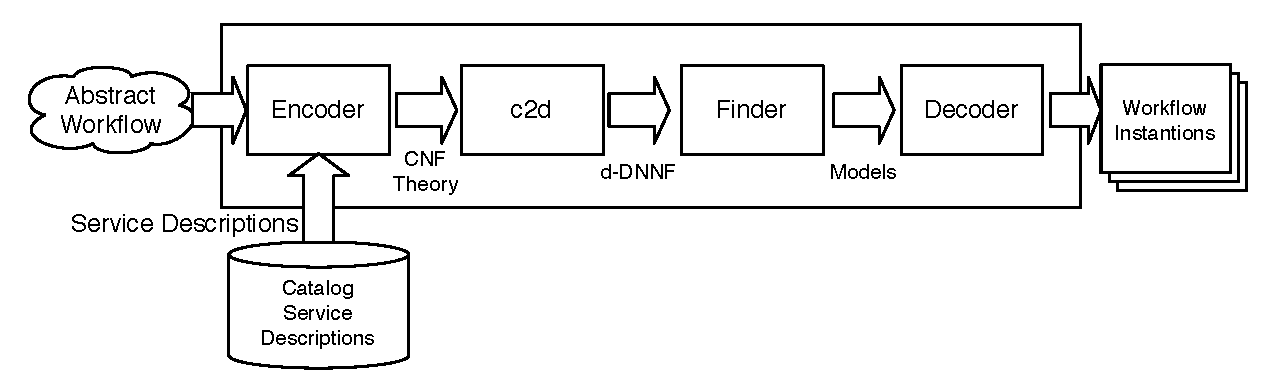
\includegraphics[width=.9\textwidth]{graphics/architecture}
\caption{Arquitectura del Sistema}
\label{fig:architecture}
\end{figure}

Se utiliza una arquitectura comprendida por un catálogo de descripciones de
servicio, el Codificador, el compilador c2d, el Buscador de mejores modelos, y
el Decodificador. La figura~\ref{fig:architecture} muestra la arquitectura global del sistema.
En esta infraestructura, una instancia del problema de instanciación de flujos
de trabajo se define como un flujo abstracto representado por una consulta
conjuntiva sobre servicios abstractos que es dada como entrada junto con un
conjunto de servicios concretos definidos por vistas de servicios abstractos.

El catálogo se pobla con descripciones de servicios abstractos y concretos; cada
servicio es descrito en términos de atributos de entrada y salida y anotado con
un valor real que representa la utilidad QoS del servicio. La descripción de los
servicios concretos, que son definidos como vistas de los servicios abstractos,
puede ser generada de manera semiautomática o automática usando herramientas
tales como el sistema DEIMOS \cite{AmbiteISWC09}.

Una instancia de entrada de WIP es codificada como una teoría CNF cuyos modelos
corresponden a las intanciaciones del flujo de trabajo por el Codificador. El
compilador c2d, un componente \emph{off-the-shelf}, compila la fórmula CNF a
d-DNNF. El Codificador traduce las instancias WIP en teorías CNF que luego son
convertidas en d-DNNF usando c2d. El Buscador computa un mejor modelo dados los
parámetros QoS en tiempo lineal en el tamaño del d-DNNF resultante. Es
importante remarcar que el proceso de compilación necesita ser realizado sólo
una vez ya que no depende del valor de los parámetros QoS. Así, incluso si la
compilación resulta ser costosa en términos de tiempo, este costo puede ser
amortizado dado que el d-DNNF resultante puede ser usado para conseguir mejores
instanciaciones con respecto a múltiples valores de los parámetros QoS.
Finalmente, el Decodificador traduce el mejor modelo retornado por el Buscador
a una instanciación de flujo de trabajo que resuelve el WIP.

Dado un CNF que codifica un WIP, su d-DNNF es una representación compacta de
todas las instanciaciones del flujo de trabajo. Es decir, uno puede generar de
una manera libre de \emph{backtracking} todas las instanciaciones del flujo de
trabajo. Si el usuario está interesado en una mejor instanciación dados
parámetros de QoS, entonces esta se puede computar en tiempo lineal en el tamaño
del d-DNNF. Si el usuario está interesado en todas las mejores instanciaciones,
estas pueden ser computadas en tiempo lineal en su número. Finalmente, si el
usuario está interesado en todas las instanciaciones, estas también pueden ser
computadas en tiempo lineal en su número. En los últimos dos casos, si ese
número es exponencial (en el tamaño de la entrada), la enumeración de las
instanciaciones también lo es pero esta complejidad es intrínsica al problema y
por lo tanto no puede ser evitada.

\subsection{Resultados Experimentales}

Se realizó un análisis empírico sobre tres experimentos. Todos los experimentos
fueron realizados en una máquina de escritorio con un CPU Intel Core 2 Duo de
2GHz y 4GB de memoria, y el tiempo fue medido con el comando de Unix
\emph{time}.

El objetivo de los experimentos es determinar el rendimiento de la propuesta con
condiciones variantes. El principal beneficio de la aproximación propuesta es
que se puede compilar la teoría lógica para una instancia del problema y luego
calcular todas las instanciaciones, o las mejores, cualquier número de veces. El
modelo de costos para conseguir mejores instanciaciones puede ser cambiado sin
necesidad de recompilar la teoría lógica. Por lo tanto, la complejidad en tiempo
de la aproximación es básicamente el tiempo para codificar el WIP como un
CNF más el tiempo para compilar el CNF en un d-DNNF y el tiempo para decodificar
los modelos. Los tiempos para codificar y decodificar son despreciables
comparados con el tiempo para compilar el CNF. Por esto, el enfoque es en el tiempo
necesario para compilar los problemas de los experimentos.

El primer experimento consiste de problemas para consultas para viajes aéreos.
Los servicios concretos son de la forma $V_i(x,y)\qrule\ \flight(x,y,\AL_i)$
donde $\AL_i$ es una
constante que denota el nombre de una aerolínea, y $\flight(x,y,\AL_i)$ relaciona las
ciudades $x$ e $y$ tales que hay un vuelo entre $x$ e $y$ servido por $\AL_i$.
Se supone que este servicio concreto retorna todos los vuelos entre dos ciudades
con una aerolínea específica. El flujo de trabajo tiene la forma

\[ W(x_1,\ldots,x_n)\ \qrule\ \flight(\PA,x_1,z),\,\flight(x_1,x_2,z),\,\ldots,\,\flight(x_n,\NY,z)\,. \]

\begin{figure}[t]
\centering
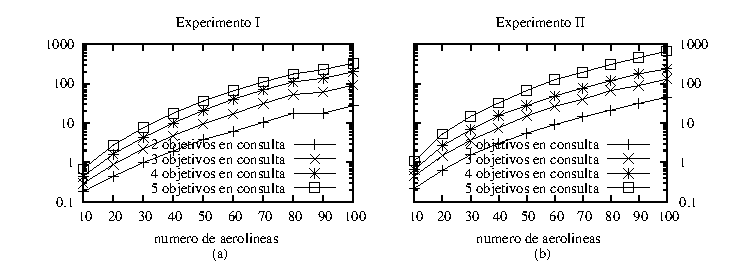
\includegraphics[width=1\textwidth]{graphics/plot1}
\caption{Tiempos de compilación para los experimentos I y II para diferentes
números de objetivos y de vistas. Los gráficos están en escala logarítmica, y el
tiempo es en segundos.}
\label{fig:plot1}
\end{figure}

El experimento incluye instancias para flujos de trabajo con 2 a 5 subobjetivos
y conjuntos de 10 a 100 servicios concretos. Los resultados para la compilación
son mostrados en el panel (a) de la figura ~\ref{fig:plot1}. Este es un gráfico en escala
logarítmica que sugiere comportamiento sub-exponencial. En cualquier caso, los
resultados muestran buen rendimiento dado que instancias realísticas del
problema (conjuntos de 100 aerolíneas con vuelos de cinco paradas) pueden ser
compiladas en 328 segundos. El tamaño en disco del d-DNNF para 100 aerolíneas y
vuelos con cinco paradas es 3,4MB. En este d-DNNF, el mejor modelo puede ser
computado en 0.29 segundos, y la enumeración de todos los modelos en 0.47
segundos.

En un intento de inducir crecimiento exponencial en el tamaño de compilación, en
el segundo experimento se agrega un segundo servicio concreto para cada
aerolínea. Esta modificación incrementa el número de instanciaciones válidas de
lineal a exponencial dado que cada tramo de un vuelo puede ser ahora instanciado
por dos servicios concretos y entonces un vuelo con $n$ tramos puede tener hasta
$2^n$ instanciaciones. Se corrió el compilador para instancias que comprendían
el mismo número de objetivos del flujo de trabajo y el número total de
servicios concretos. Los resultados graficados en escala logarítmica se muestran
en el panel (b) de la figura ~\ref{fig:plot1}.

Estas pruebas muestran buen rendimiento para este tipo de problemas, pero no
involucran servicios concretos con múltiples objetivos. Por lo tanto se
diseñó un tercer experimento que consiste de instancias no estructuradas y
generadas aleatoriamente. Cada instancia contiene tres variables por servicio
abstracto, diez variables distintas y diez constantes distintas, seis
objetivos en los flujos de trabajo, 2 a 5 objetivos en los servicios
concretos, y número de servicios variante. La probabilidad de que un argumento
de un servicio abstracto esté ligado a una constante es 50\%. Los resultados se
muestran en la figura ~\ref{fig:plot3}. El tiempo de compilación de estas instancias no
crece monótonamente dado que son generadas aleatoriamente. Lo mismo ocurre para
el tamaño de las teorías y los números de modelos. Por ejemplo, el d-DNNF para
un problema con 45 vistas cada una con 5 objetivos fue de tamaño 5,1Mb y tuvo
$1.26\times 10^8$ modelos. El tiempo para buscar el mejor modelo para este
d-DNNF es 0.46 segundos mientras que el tiempo para enumerar todos los modelos
es alredededor de 17 horas.

\begin{figure}[t]
\centering
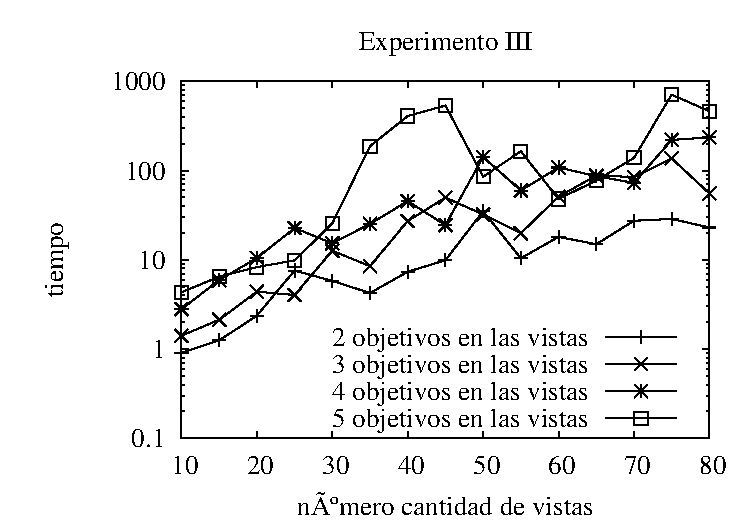
\includegraphics[width=.8\textwidth]{graphics/plot3}
\caption{Tiempos de compilación para el experimento III para diferentes números
de objetivos y de vistas. Los gráficos están en escala logarítmica, y el
tiempo es en segundos.}
\label{fig:plot3}
\end{figure}

Estos son experimentos preliminares, pero los resultados muestran que la
aproximación propuesta escala eficientemente para problemas con varios objetivos
y vistas. Se cree que estos resultados son alentadores y motivan a continuar
esta línea de investigación.


\addcontentsline{toc}{section}{Referencias} 
\bibliographystyle{abbrv}
\bibliography{ref}

\end{document}
